%src/kmvEquations.tex
%
\section{KMV Equations}
We do implement a variant of the KMV sketch in the Sketch Library called the QuickSelect sketch. The subtle differences between the conventional definition of the KMV sketch and the QuickSelect sketch is summarized at the end. This derivation is similar to that of Giroire\cite{Giroire2009}, but is more direct and includes rudimentary steps that Giroire omits.
%
\subsection{Preliminaries}
%%%%%%%%%%%%%%%%%%%%%%%%%%%%%%%%%
\subsubsection{Uniform Probability Density and Distribution}
%
\begin{figure*}
\begin{center}
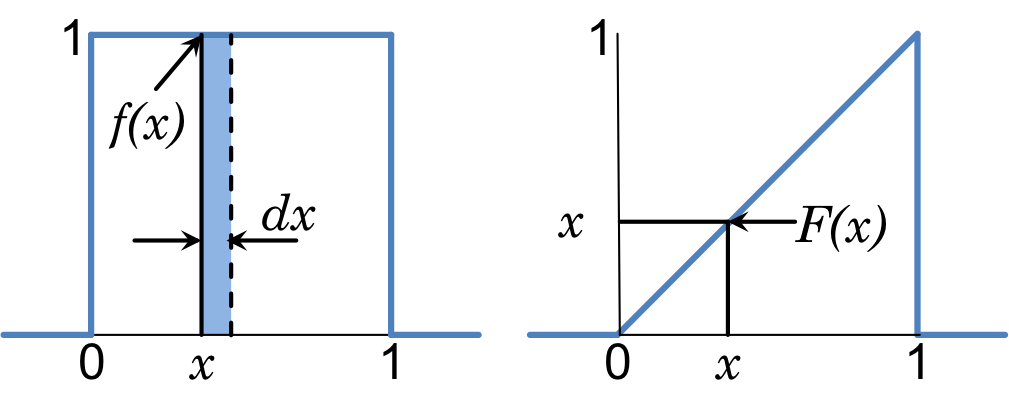
\includegraphics[width=0.5\linewidth]{figures/UniformDenCum.png}
\end{center}
\caption{Uniform density (left) and distribution (right)}
\end{figure*}
%
One of the fundamental concepts of sketches is that the raw input stream of 
unique values is transformed into a stream of unique hash values that have 
a uniform random distribution. 
This is accomplished internally by a hash function that has good avalanche 
and bit-independence properties.  
%(Further discussion of this hash function is out-of-scope for this paper.)

We begin by defining a continuous uniform random variable $X$ on the interval
[0,1]:
\begin{align}
\shortintertext{The Prabability Density Function (PDF) (Figure 1, left):}
f(x)            &= \begin{cases}
                     1  & 0<x<1   \\
                     0  & \text{otherwise} 
                   \end{cases}  \label{density} \\
\int_0^1 f(x)dx &= 1 \notag \\
f(x_0)          &= P(x = x_0) \notag \\
\shortintertext{The Cumulative Distribution Function (CDF) (Figure 1, right):}
F(x_0)          &= P(x<x_0) \notag \\
                &= \int_0^{x_0} f(x)dx=x_0 \label{distribution}
\end{align}

%%%%%%%%%%%%%%%%%%%%%%%%%%%%%%%%%
\subsubsection{Expected Value of \texorpdfstring{$g(x)$}{g(x)} Given Density \texorpdfstring{$f(x)$}{f(x)}}
Given a random variable $X$ with a density function $f(x)$, and another 
function of $X$, $g(x)$, 
the expected value of $g(x)$ is given by the inner product of $f$ and $g$. 
See \href{https://en.wikipedia.org/wiki/Expected_value}
{Wikipedia Expected Value} and Appendix A for a discrete example.
\begin{align}
E[g(x)] = \int_0^1 g(x)f(x)dx \label{EV}
\end{align}
%%%%%%%%%%%%%%%%%%%%%%%%%%%%%%%%%
\subsubsection{Euler Beta Function}
The Euler Beta function is a special function that has different forms 
that can be very useful depending on the context.
It is particularly useful in solving the integrals that occur in Order 
Statistics by converting the integrals into Gamma or Factorial expressions.
\begin{align}
\shortintertext{For $\mathbb{R}(a), \mathbb{R}(b) > 0$}
\B(a,b)    &= \int_{t=0}^1 t^{a-1} (1-t)^{b-1}dt \label{betaIntegral} \\
          &= \frac {\Gamma(a)\Gamma(b)}{\Gamma(a+b)} \notag\\
\shortintertext{For integers $a, b > 0$}
\Gamma(a) &= (a-1)! \notag \\
\B(a,b)    &= \frac{(a-1)!(b-1)!}{(a+b-1)!} \label{betaFactorial}
\end{align}
%
%
%%%%%%%%%%%%%%%%%%%%%%%%%%%%%%%%%
\subsubsection{The \texorpdfstring{$k^{th}$}{Kth} Order Statistic, part 1}
We start with a set of $n$ labeled random variables $X_1,\dots,X_n$ in the 
interval $[0,1]$ that have a density $f(x)$ and a distribution $F(x)$.
If we take one instance of all the $X's$, we can order them and identify 
them by their order 
$X_{(1)}, \dots, X_{(n)}$, which is independent of the labels.
Our goal is to find the density function and expected value of the 
$k^{th}$ minimum value (KMV), $M_{(k)}$. 
This analysis only assumes that the underlying probability density of the 
$X's$ is a real analytic function. 
At the end of the analysis we simplify to the uniform random density case.
%
\begin{figure*}[b]
\begin{center}
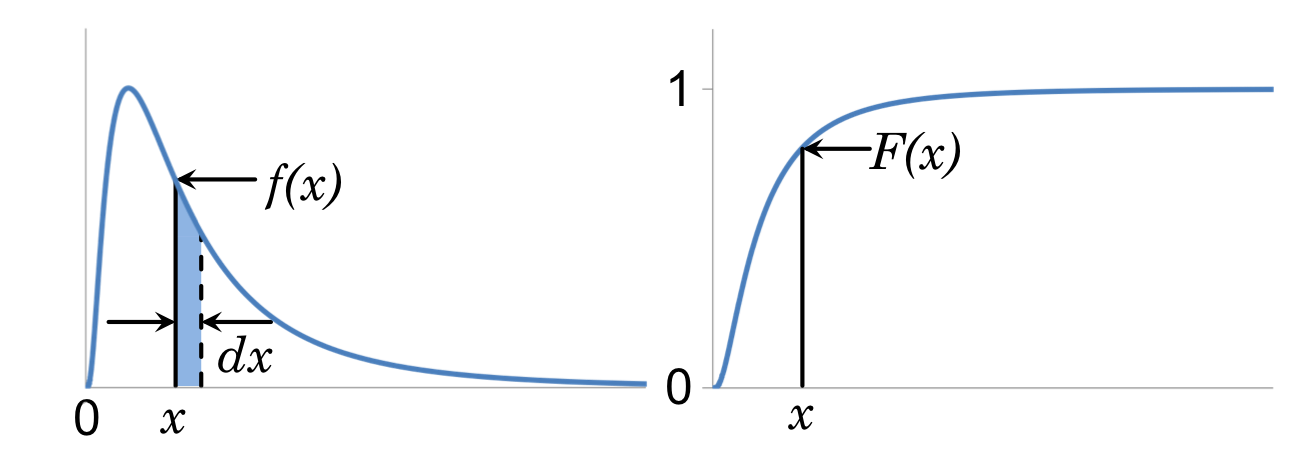
\includegraphics[width=0.5\linewidth]{figures/LogNormDenCum.png}
\end{center}
\caption{Some arbitrary density (left) and distribution (right)}
\end{figure*}
%
\begin{align*}
\shortintertext{The density of $M_{(k)}$ (Figure 2)}
f_{(k)}(x)dx &= P(M_{(k)} \in dx) \\
             &= P(\text{exactly one of } X's \in dx,\text{exactly } k-1 \text{ of }X's < x)
\shortintertext{There are $n$ $X's$, each with the same $f(x)$.}
               &= P(X_1 \in dx, \text{exactly } k-1 \text{ of the other }X's < x) + \\
               &\phantom{{}=\ }P(X_2 \in dx, \text{exactly } k-1 \text{ of the other }X's < x) + \\
               &\phantom{{}=\ }\dots + \\
               &\phantom{{}=\ }P(X_n \in dx, \text{exactly } k-1 \text{ of the other }X's < x). \\
               &\phantom{{}=\ } \\
f_{(k)}(x)dx   &= nP(X_1 \in dx, \text{exactly } k-1 \text{ of the other }X's < x) \quad \text{choice of $X_1$ is arbitrary}
\end{align*}
\begin{align*}
\shortintertext{From probability theory.}
P(X_1 \in dx)                        &= f(x)dx \\
P(\text{at least } (k-1) X's < x)    &= (F(x))^{k-1} \\
P(\text{at least } (n-k) X's > x)    &= (1-F(x))^{n-k} 
\shortintertext{Note that there are $\binom{n-k}{k-1}$ combinations of $(k-1)$ $X's < x$.}
\end{align*}
%
%
To force exactly $(k-1)$ $X's < x$ we partition the probability space into three parts: 
$X\in dx, X<x, X>x+dx$.
\begin{align*}
f_{(k)}(x)dx &= n\quad f(x)dx \quad \binom{n-1}{k-1} (F(x))^{k-1} \quad (1-F(x))^{n-k}\\ 
\end{align*}
Let's simplify the above by assuming the uniform random probability density instead of an arbitrary density.
Recall that $f(x_0)=1$ and $F(x)=x_0$ from \ref{density} and \ref{distribution}. 
\begin{align}
f_{(k)}(x)dx &=n\binom{n-k}{k-1}x^{k-1}(1-x)^{n-k}dx \notag \\
             &=k\binom{n}{k}x^{k-1}(1-x)^{n-k}dx \label{kthOrderDensity} \\
\shortintertext{The Expected Value of $M_{(k)}$ becomes}
E[M_{(k)}]   &= \int_0^1 (x)\left[k\binom{n}{k}x^{k-1}(1-x)^{n-k}\right]dx \notag\\
             &= k\binom{n}{k} \int_0^1 x^{k}(1-x)^{n-k}dx \label{integral1}
\end{align}

%%%%%%%%%%%%%%%%%%%%%%%%%%%%%%%%%
\subsubsection{The \texorpdfstring{$k^{th}$}{Kth} Order Statistic, part 2: Using the Beta Function }
The integral of \ref{integral1} can be recognized as a form of the Beta integral from \ref{betaIntegral}.
%
\begin{align}
\shortintertext{Let $a=k+1$, $b=n-k+1$, $a+b = n+2$}
\B(k+1,n-k+1) &= \int_{t=0}^1 t^{k}(1-t)^{n-k}dt, \notag \\
\shortintertext{and the Beta factorial form from \ref{betaFactorial}}
             &= \frac{k!(n-k)!}{(n+1)!}. \notag 
\shortintertext{This means that \ref{integral1} can be written}
E[M_{(k)}]   &= k\binom{n}{k}\B(k+1,n-k+1) \notag \\
             &= k\binom{n}{k} \frac{k!\ (n-k)!}{(n+1)!} \notag \\
             &= \frac{k\ n!}{k!(n-k)!}\frac{k!\ (n-k)!}{(n+1)!} \notag \\
E[M_{(k)}]   &= \frac{k}{n+1} \label{evKMV}
\end{align}


%%%%%%%%%%%%%%%%%%%%%%%%%%%%%%%%%
\subsection{The Expected Value of the Inverse of \texorpdfstring{$M_{(k)}$}{M(k)}}
In order to estimate $n$ we need to derive $E[\frac{1}{M_{(k)}}]$.
From \ref{EV} and \ref{kthOrderDensity} we have
\begin{align}
E\left[\frac{1}{M_{(k)}}\right] &= \int_0^1 \left(\frac{1}{x}\right)\left[k\binom{n}{k}x^{k-1}(1-x)^{n-k}\right]dx     \notag \\
                               &=k\binom{n}{k} \int_{x=0}^1 x^{k-2}(1-x)^{n-1}dx.           \label{integral2}
\shortintertext{Again using the Beta integral and factorial forms from \ref{betaIntegral} and \ref{betaFactorial} for the integral in \ref{integral2}:}
\shortintertext{Let $a=k-1, b=n-k+1, a+b=n$}
\B(k-1, n-k+1)                  &= \int_{t=0}^1 t^{k-2}(1-t)^{n-k}dt                         \notag \\
                               &= \frac{(k-2)!(n-k)!}{(n-1)!}                               \label{inverseFactorial}
\shortintertext{Substituting \ref{inverseFactorial} into \ref{integral2}:}
E\left[\frac{1}{M_{(k)}}\right] &= k\binom{n}{k} \B(k-1,\ n-k+1)                              \notag \\
                               &= \frac{k\ n!}{(n-k)!\ k!}\frac{(k-2)!\ (n-k)!}{(n-1)!}     \notag \\
E\left[\frac{1}{M_{(k)}}\right] &= \frac{n}{k-1}                                              \label{inverseExpectation}
\shortintertext{We don't know $n$. What we want is $\hat{n}$, an asymptotically unbiased estimate of $n$.}
\shortintertext{Solving \ref{inverseExpectation} for $n$ it becomes the estimate, $\hat{n}$}
\hat{n}                        &= (k-1)\left(\frac{1}{M_{(k)}}\right) = \frac{k-1}{M_{(k)}}         \label{nhat} \\
E[\hat{n}]                     &= (k-1)E\left[\frac{1}{M_{(k)}}\right] = (k-1)\frac{n}{k-1} = n.    \label{EVn}
\end{align}
This proves that our estimate of $n$ is indeed unbiased.


%%%%%%%%%%%%%%%%%%%%%%%%%%%%%%%%%
\subsection{The Variance of \texorpdfstring{$\hat{n}$}{est(n)}}
From the expected value of $\hat{n}$ from \ref{EVn} we have: 
\begin{align}
E[\hat{n}]        &= n \notag \\
\shortintertext{The variance of $\hat{n}$ }
\sigma^2[\hat{n}] &= E[\hat{n}^2] - E[\hat{n}]^2 = E[\hat{n}^2] - n^2 \notag 
\end{align}
%
\begin{align*}
\shortintertext{Evaluating the term, $E[\hat{n}^2]$ by squaring \ref{EVn}:}
E[\hat{n}^2] &= (k-1)^2 E\left[\left(\frac{1}{M_{(k)}}\right)^2\right] \\
%\end{align*}
%
%\begin{align*}
\shortintertext{Evaluating the term, $E\left[\left(\frac{1}{M_{(k)}}\right)^2\right]$}
E\left[\left(\frac{1}{M_{(k)}}\right)^2\right] &= \int_0^1 \left(\frac{1}{x^2}\right)\left[k\binom{n}{k}x^{k-1}(1-x)^{n-k} \right]dx \\
                                             &= k\binom{n}{k} \int_0^1 x^{(k-2)-1}(1-x)^{(n-k+1)-1}dx \\
\shortintertext{Again using the Beta integral and factorial forms from \ref{betaIntegral} and \ref{betaFactorial}:}
\shortintertext{Let $a=k-2, b=n-k+1, a+b=n-1$}
                                             &= k\binom{n}{k} \B(k-2, n-k+1) \\
                                             &= \frac{k\ n!}{(n-k)!\ k!} \frac{(k-3)!\ (n-k)!}{(n-2)!} \\
E\left[\left(\frac{1}{M_{(k)}}\right)^2\right]  &= \frac{n\ (n-1)}{(k-1)\ (k-2)} 
%\end{align*}
%
%\begin{align*}
\shortintertext{Returning to the evaluation of $E[\hat{n}^2]$:}
E[\hat{n}^2]                                 &= (k-1)^2 \frac{n\ (n-1)}{(k-1)\ (k-2)} \\
                                             &= \frac{n\ (n-1)\ (k-1)}{(k-2)} \\
\shortintertext{Returning to the evaluation of $\sigma^2[\hat{n}]$}
\sigma^2[\hat{n}]                            &= \frac{n\ (n-1)\ (k-1)}{(k-2)} - n^2 \\
                                             &= \frac{n\ (n-1)\ (k-1) - (k-2)\ n^2}{k-2} \\
\sigma^2[\hat{n}]                            &= \frac{n^2-n(k-1)}{k-2} < \frac{n^2}{k-2}
\end{align*}
%
Normalizing the variance by $n^2$ and taking the square root results in the Relative Standard Error (RSE):
\begin{align}
RSE[\hat{n}] = \sqrt{\frac{\sigma^2}{n^2}} &= \sqrt{\frac{1}{k-2} - \frac{k-1}{n(k-2)}} < \frac{1}{\sqrt{k-2}} \label{rse} \\
RSE[\hat{n}]_{n \to \infty}             &= \frac{1}{\sqrt{k-2}}
\end{align}
This proves that the RSE is always less than a constant!
%
%%%%%%%%%%%%%%%%%%%%%%%%%%%%%%%%%
\subsection{Equation Differences Between KMV and QuickSelect}
Much of the research literature on KMV sketches defines a cache of size $k$ that holds the $k^{th}$ minimum value ($M_{(k)}$) and $k-1$ hash values less than $M_{(k)}$.  
The Theta Sketch Framework (TSF), however, is more flexible and different from the standard KMV definition.
In the TSF, the label $k$ is used as a user configured parameter that defines the maximum RSE for the sketch. 
Instead of $M_{(k)}$ being a member of the cache array of hash values, 
TSF sketches have a separate register called $\theta$ and define different Theta Choosing Functions (TCF) algorithms for computing $\theta$ for different sketch families. 
See \href{http://datasketches.github.io/docs/ThetaSketchFramework.pdf}{Theta Sketch Framework}.

This requires minor changes to the above equations for the QuickSelect family.
\begin{equation*}
\arraycolsep=15pt
\renewcommand\arraystretch{1.5}
\begin{array}{lll}
\text{Ref / Equation}                                           & \text{KMV}                       & \text{QuickSelect}\\
\text{TCF}(\theta) =                                            & M_{(k)}                             & M_{(k+1)}\\
\ref{evKMV} \quad E[\theta] =                            & \frac{k}{n+1}                     & \frac{k+1}{n+1}\\ 
\ref{inverseExpectation} \quad E\left[\frac{1}{\theta}\right] = & \frac{n}{k-1}   & \frac{n}{k}\\
\ref{nhat} \quad \hat{n} =                                    & \frac{k-1}{\theta}               & \frac{k}{\theta}\\
\ref{rse}  \quad RSE(\hat{n})\leq                         & \frac{1}{\sqrt{k-2}}            & \frac{1}{\sqrt{k-1}}\\
\end{array}
\end{equation*}